\documentclass[11pt]{article}
\usepackage{cite}
\usepackage[useregional]{datetime2}
\usepackage{babel}
\usepackage{graphicx}

\usepackage{dirtytalk}
\usepackage{geometry}
\geometry{
    a4paper,
    total={170mm,257mm},
    left=20mm,
    %right=40mm,
    top=20mm,
    marginparsep=-7mm,
    marginparwidth=20mm
}


\usepackage{setspace}
\doublespacing

% shrink marginpar font size
\let\oldmarginpar\marginpar
\renewcommand\marginpar[1]{\-\oldmarginpar[\raggedleft\footnotesize #1]%
{\raggedright\footnotesize #1}}

\begin{document}

\title{Understanding and Avoiding AI Failures: A Practical Guide}
\author{Max Williams \\ University of Louisville \and Roman Yampolskiy \\ University of Louisville}
\date{\today}
\maketitle

\abstract{
    In place of root cause analysis, we look over the history of AI catastrophes to find common
    themes between these failures to develop a rudimentary guide as to what failures to expect based
    on the nature of a technology and means to mitigate the damage or a recommendation to
    unilaterally discontinue research in extreme cases. By focusing on thematic analysis instead of
    root cause, we can systematically identify when and where attention should be paid to safety of
    current generation AI systems.}

\section{Introduction}

With current AI technologies, harm done by AIs is limited to power that we directly put in their
hands.  As said in \cite{yam2018historic}, ``For Narrow AIs, safety failures are at the same level
of importance as in general cybersecurity, but for AGI it is fundamentally different.'' Despite AGI
still being well out of reach, the nature of AI catastrophes has already changed in the past two
decades. Automated systems are now not only malfunctioning in isolation, they are interacting with
humans and with each other in real time. This shift has made traditional systems analysis impossible,
as the other entities interacting with any given AI are neither homogeneous nor rational.

In response to this, we analyze how risks associated with complex control systems has been managed
historically and contemporary AI failures to create a framework for predicting what kinds of risk
are created from the operation of any AI system. We create a framework for analyzing AI systems
before they fail to understand how they change the risk landscape of the systems they are embedded
in.

\section{Terminology}

Systems accident: An accident in a system with high complexity and tight coupling caused by complex
interactions between system components. They are often incomprehensible to operators.
\cite{perrow1999living}

Normal accident: Synonym for Systems Accident. ``Normal" here refers to the inevitability of the
accident from the system's functioning often despite best efforts to avoid an accident.

Tight coupling: Two components are tightly coupled if one depends on the other, especially if this
dependence happens on a very short time scale.

Loose coupling: Two components are loosely coupled if one depends on the other indirectly or if there
is a lot of time in the interaction

Slack: Redundancy and time for errors to be noticed both create slack. Highly redundant systems are
often designed with lots of slack, which is used up as components degrade over time or under
stress. Slack also refers to the divergence of mnetal models used by operators, creating mental
redundancy that makes it more likely that a problem is solved correctly.

\section{Related work}


Risk of failure is a property inherent to complex systems, and complex systems are inherently
hazardous \cite{cook1998complex}.  At a large enough scale, any system will produce ``Normal
Accidents''. These are unavoidable accidents caused by a combination of complexity, coupling between
components, and potential harm. A normal accident is different from the more common component
failure accidents in that the events and interactions leading to normal accident are not
comprehensible to the operators of the system \cite{perrow1984living}. Increasing the complexity
and broadening the role of AI components in a system decreases comprehensibility of the system,
leading to an increase in normal accidents.

As computer control systems increased in complexity in the 70's and 80's, unexpected and sometimes
catastrophic behaviour would emerge from previously stable systems \cite{anderson2005control}. While
linear control systems had been used for some time (for example, a thermostat) without unexpected
behaviour, adaptive control systems created novel and unexpected problems, such as ``bursting''. As
described in \cite{anderson2005control}, bursting is the phenomenon where a stable controller would
function as expected for a long time before bursting into oscillation, then returning to a stable
state. This is caused by the adaptive controller not having a rich enough input during the stable
period to determine the unknown coefficients of its model correctly, causing the coefficients to
drift. Once the system enters oscillation, the signal again becomes rich enough for the controller
to correctly estimate the unknown coefficients and the system becomes stable again. The increased
complexity of the more advanced technology (dynamic controller instead of a  static controller)
introduced a dynamic not present in previous technologies, and incomprehensible to an operator not
familiar with this behavior. Worse, since this behavior only happens when the controller is
controlling the real world plant, designers had no way of predicting this failure mode. Bursting can
be reduced using specifically engineered safety measures or more complex controllers (which bring
even harder to understand problems), but still demonstrates that increases in complexity always
bring risk.

The introduction of lethal autonomous weaponry \cite{carvin2017normal} increases the danger of
normal accidents not because it provides new kinds of failure or novel control system but because of
the drastically increased potential harm. A machine which kills when functioning
correctly is much more dangerous in an accident than one which only does harm when malfunctioning.
By increasing the level of complexity and autonomy of weapons systems, normal accidents involving
powerful weapons becomes a possibility.

\subsection{Normal Accident Theory}

In 1984, Charles Perrow published ``Normal Accidents" \cite{perrow1984living} which laid the
groundwork for NAT (Normal Accident Theory). Under NAT, any system that is tightly coupled
and complexly interactive will inevitably experience a systems accident. Decentralization reduces
coupling and increases complexity, while centralization decreases complexity but also increases
coupling. Thus, since an organization cannot be both centralized and decentralized, large
organizations will harbor system properties that make them prone to normal accidents.

\subsection{High Reliability Theory}

% quote of the day: One of the principal values of `normal accident' analysis and case descriptions
% is that it helps to develop convincing materials to counter the naive, perhaps wistful or
% short-sighted, views of descision-makers who, due to institutional  presssure, desperation or
% arrogance, are temped to make unrealistic assumptions about the systems they direct but for which
% they have only nominal operational responsibility. 
% https://onlinelibrary.wiley.com/doi/10.1111/j.1468-5973.1994.tb00045.x

High reliability theory was developed to explain the incredible ability of certain organizations to
function without major accidents for long periods of time. In \cite{weick1999reliability}, Weick
identifies several common traits shared by high reliability organizations (HROs): a strategic
prioritization of safety, careful attention to design and procedures, a limited degree of
trial-and-error learning, redundancy, decentralized decision making, continuous training often
through simulation, and strong cultures that encourage vigilance and responsiveness to potential
accidents.  

% This is off topic but it struck me as important so I'm leaving it in for now
High reliability organizations manage the apparent paradox proposed in normal accident theory by
having traits of both centralization and decentralization. Decision making is decentralized,
allowing for decoupling while policy and cultural factors are highly centralized, allowing for the
unification of goals and attention to safety. This ability to be simultaneously centralized and
decentralized through common culture and goals is present not only in HROs but many post-industrial
societies as identified by Hofstadter in [TODO cite, or maybe delete this paragraph as being
off-topic]

\subsection{NAT-HRT merger}

Normal accident theory holds that for certain kinds of industries systems accidents are inevitable.
Meanwhile, high reliability theory makes the observation that there are many exceptions to this, and
there are common traits shared by these ``high reliability organizations" (HROs) that can be studied
and understood as indicators of reliability. In \cite{shrivastave2009normal}, Shrivastava et al
analyze works which frame these two theories as being in conflict then reconcile the two theories.

Normal accident theory states that a system has to choose to trade off between centralization (which
allows for organization-aligned action and less chaos) and decentralization (which allows and
enables operators to quickly make decision). High reliability theory considers that it is possible
to escape this apparent paradox by allowing operators a high level of autonomy (decentralized
decision making) while also putting a focus on cultural aspects that improve safety and reliability
(centralized goals).

Shrivastava et al bring in the Swiss cheese model (SCM) to explain the importance of time in the
occurrence of accidents, even in systems that are stable over time. In the SCM, the layers of safety
are modeled as slices of cheese with holes in them representing weak points in each layer of safety.
Over time, holes change shape and move around. Eventually, no matter how many slices of cheese
(layers of safety) there are, the holes will align allowing a straight shot through all of the
slices of cheese [TODO cite Reason, 1998]. However, the SCM model only helps understand that
accidents are inevitable, and ``inevitability is immaterial for practical purposes" as Shrivastava
et al state, since the time scales involved for some systems may be too great to consider possible.

Disaster incubation theory (DIT) is also introduced as the final piece needed to reconcile normal
accident theory and high reliability theory. DIT describes how organizations gradually migrate to
the boundary of acceptable behavior, as good safety records drive up complacency and deviance is
normalized [TODO cite Vaughan 2005, Rasmussen, 1997]. DIT was considered only useful in hindsight by
proponents of NAT, so Snook [TODO cite Snook 2000] investigated accidents with this in mind and
created the framing of ``practical drift". This is the `slow steady uncoupling of local practice
from written procedure' which leads an initially highly coupled system to become uncoupled from
operators and managers optimize their processes to be more efficient, deviating from procedure.
Then, if the system is required to become tightly coupled again, the operators are ill-prepared for
this increase in coupling and systems accidents become far more likely.

Through the lens of disaster incubation theory and practical drift, Shrivastava et al explain how
NAT and HRT actually work to compliment each other to explain how accidents take place and are
avoided. The time period being considered by HRT takes place while the system is still a high
reliability organization. The culture and procedures put in place are working correctly, coupling is
high and complexity is manageable to the well trained operators. Over time, however, practical drift
decouples the system, and reliability decreases. If the organization is a high reliability
organization, degradation is limited and incidents can still be managed. Accidents that take place
during this period of time are within the scope of HRT. However, there is the possibility for an
unlikely event to lead from this steady decline of reliability into the normal accident of NAT. If
the system suddenly has to become more coupled (for instance, during a special mission or to react
to an incident breaking down multiple layers of safety mechanisms), it is ill prepared to do so. At
this point, NAT's trade-off between coupling and complexity becomes important, and the perceived
complexity of the system increases drastically, making safe operation impossible, leading to a
normal accident. This can only happen after a great decrease in coupling from the initial (designed)
state of the system, so proponents of HRT would say that the accident was only able to take place
due to the system no longer acting as a high reliability organization. 

Thus high reliability theory can serve to understand how organizations resist practical drift, and
the accidents that happen when practical drift leads to accidents. Normal accident theory is useful
when practical drift has lead to a great degree of decoupling, then a sudden change in situation
(which may be an intentional operation or an incident) leads to the need to increase coupling, which
the system is (surprisingly, to operators) no longer able to handle without increasing complexity
beyond manageable levels. 

\subsection{???}

In \cite{uesato2018adversarial}, Jonathan Uesato et al show that by training a reinforcement learner
in an environment with adversarial perturbations instead of random perturbations, failure modes that
would be extremely unlikely to be encountered otherwise were detected and integrated into training.
This shows that AI trained to be ``robust'' by training in a noisy environment may have catastrophic
failure modes that are not observed during training but can spontaneously occur after deployment in
the real world. Adversarial training is a tool to uncover and improve these issues, but is only an
engineering safety measure over the deeper issue of black box AI which are not characterized of
their entire input space.

Large collections of AI failures and systems to categorize them have been created before
\cite{yam2018historic} \cite{scott2020classification}. In \cite{scott2020classification}, the
classification schema details failures by problem source (such as design flaws, misuse, equipment
malfunction, etc.), consequences (physical, mental, emotional, financial, social, or
cultural), scale of consequences (individual, corporation, or community), and agency (accidental,
negligent, innocuous, or malicious). It also includes preventability and software development
life-cycle stage.

The proliferation of AI technologies has impacts in our socioeconomic systems and environment in
complicated ways, both positive and negative \cite{jayden2018sustainability}. AI has the ability to
make life better for everyone but also to negatively impact many by displacing workers and
increasing wealth disparity [TODO find a citation that isn't a news source]. This is just one
example of AI interacting with a complicated system (in this case, the job market) to have large
scale consequences. 


\section{Classification schema for AI systems}
\label{sec:classification}

We present a tags based scheme adapted from the one presented in \cite{scott2020classification}.
Instead of focusing on AI failures, this schema classifies the AI systems themselves, allowing for
risk analysis prior to failure or additional failures of the system. We pay particular attention to
the orientation of the AI system as both a system with its own components prone to failure and a
component in a larger system which depends on the AI to some degree. Any analysis attempting to
divide a system into components must acknowledge the `ambiguities, since once could argue
interminably over the dividing line between part, unit, and subsystem' \cite{perrow1999living}.
\marginpar{TODO read \cite{perrow1999living} so I'm not poaching this citation from
\cite{shrivastave2009normal}}

To characterize the risk of an AI system, one of the most important factors is identifying the
larger system in which the AI is a component. In an experimental setting, a genetic algorithm
hacking the simulator can be an amusing bug \cite{lehman2018surprising}, but a similar bug making
its way into an autonomous vehicle or industrial control system would be potentially extremely
dangerous. We look at the way an AI system is used as a component in three ways: (1) the intended
use of the AI, (2) the way the AI is marketed, and (3) the way the AI is actually being implemented.
Disparity between (1) and (2) can be caused by hype among those seeking profit from AI and poor
communication between engineers and salespeople. Disparity between (2) and (3) can be caused by
ignorance on the part of the buyer, lack of accessible instructional material, and intentional
off-label use where the AI is good enough at the task despite not being designed for it. (TODO go on
to argue that this separation between AI design by engineers and AI implementation is very common
and a notable contributor to failure of AI systems acting as components in larger systems)

At the current technological scale, AI are not dangerous in isolation [TO CITE]. Their outputs must
be connected to some means of control. This can take many forms: indirectly, with AI informing humans
who then make decisions, or directly with an AI controlling the actuators of a robot or chemical
plant. Any useful AI system has some degree of control over the world, and it may not be clear where
the effects of the AI take place. This connection, where the output of a component (the AI) has
significant effects on other components or system properties is an instance of coupling. Because
there are multiple components affected by the AI and those components are themselves coupled with
other components, we frame this problem in terms of the AI and a `target' which the AI can affect.
For example, an AI meant to control the flow speed of a dam controls electrical signals from itself
to the flow regulator, the actuators of the flow regulator, the flow speed of the water, and the
volume of water deposited downstream in an interval of time. All four angles have unique
consequences the might be overlooked in analyzing just one of these targets.

Observability of the warning signs of an accident is important as it allows for interventions by
human operators, a crucial tool in preventing accidents (``People continuously create safety''
\cite{cook1998complex}). The likelihood of timely human interventions depends on four things:
\begin{itemize}
    \item Time delays between AI outputs and the effects of the target.
    \item Observability of the system state as it's relevant to potential accidents.
    \item Frequency and attention paid by human operators.
    \item Ability of operators to correct the problem once it's been identified.
\end{itemize}

The time delay between an AI creating an output and that output affecting the target is essential to
preventing accidents.  Tightly coupled systems with short time delays (such as automated stock
trading) are more hazardous because the system can go from apparent normalcy to catastrophe faster
than operators can realize there is something wrong [TODO CITE the flash crash].

Observability and attention from human operators are needed for these time delays to be an effective
component of safety. As the level of automation of a system increases, human operators become less
attentive and their understanding of its behavior decreases \cite{bainbridge1983ironies}. Reliance
on automated systems decreases an operator's ability to regain control over a system if an accident
requires manual control. For example, if an autonomous driving system fails, the driver, now less
familiar with driving, has to suddenly be in manual control. Together, observability, human
attention, and human ability to correct possible failures in the system all make up a major factor
in whether or not a malfunction leads to an accident.

For a given choice of target being controlled by the AI, there is maximum conceivable amount of
damage that can be done by malicious use of that target. We use the figure as a cap as to the amount
of harm possible. Most AI failures are not malicious [TODO cite, maybe?], so the harm done by an
accident will almost always be much less than this amount. \marginpar{is maximum conceivable damage
a useful metric? It seems sound, however in many accidents, the harm is far greater than what seems
possible from the limited scope of what the AI seems to control. Multiple connected failures are
usually present at serious accidents, in a way that does more harm than either component could do on
its own}

The final criteria for classifying the nature and degree of risk of an AI system it its
interconnectivity with other system, and their degree of complexity. Loosely coupled systems have
sparse connectivity which limits the propagations of component failure into an accident, but are
also less robust. Tightly coupled systems have dense connectivity and many paths between components,
and often feedback loops that allow a component to affect itself in complicated ways [TODO cite umm
probably the original Normal Accident Theory book]. Classifying the level of coupling of the system
in proximity to the AI component can be difficult and nebulous, so only course categories (Loosely
coupled, moderately coupled, tightly coupled) are used in this analysis as finer grained
considerations are likely to become arbitrary.

[TODO where to put the quadrants thing? I'll have to weave it into the factors.]
\begin{figure}[h]
    \centering
    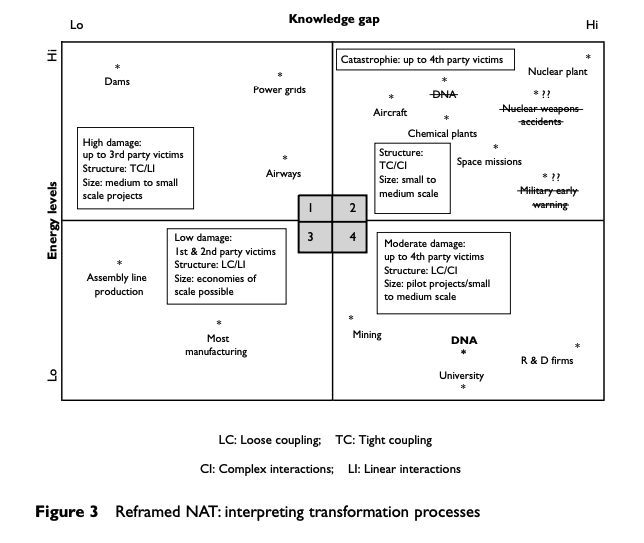
\includegraphics[width=0.25\textwidth]{images/reframed-nat-2axis}
    \caption{Plotting energy level against knowledge gap to create 4 quadrants, from
    \cite{shrivastave2009normal}}
    \label{fig:quad}
\end{figure}



The following factors are considered most significant to understanding the level and nature of
the risk of any AI system:

\begin{itemize}
    \item Disparity between design and marketing
    \item Disparity between design and usage (knowledge gap)
    \item The system which is affected by the outputs of the AI
    \item Time delay between AI outputs and the larger system
    \item System observability, level of human attention, and ability of operators to correct for
            malfunctioning of the AI
    \item The maximum damage possible by malicious use of the systems the AI controls
    \item Coupling of the components in proximity to the AI component
\end{itemize}

\subsection{Mismarketing and Off Label Use}

Mismarketing (using observed as hype) is measured on a 0-5 scale, with 1 being little or no hype and
5 being excessive hype. This can also been seen as the y axis on the famous Hype Cycle graphs
\cite{oleary2008hype}, and is also a significant factor in the ``knowledge gap" in Figure
\ref{fig:quad}. 

\subsection{Observability, Human Attention, and Correctability}

This measures how observable the internal state of the system is, how often and with what degree of
attention a human will attend to the system, and how easy or difficult a failure of the AI component
of the system is to correct once detected.

Observability is measured on a scale of 0-5, from 0 for a complete black box to 5 for AI whose
relevant inner workings can be understood at a glance.

Human Attention is measured as the number of hours in a day that an operator will spend monitoring
or investigating the AI component when there have not been any signs of malfunction. If the system is
not monitored regularly, then this is instead written as the amount of time that will pass between
checkups. This is

\subsection{Coupling}

This considers other components and aspects of the environment that the AI is coupled with.
Examples of coupling include taking data in from another component, transmitting data to another
component, relying on the functioning of a component, having another component rely on the
functioning of the AI, an aspect of the environment the AI directly or indirectly affects by its
decisions. For each coupled component, score on a scale of 1-5 from loosely coupled to strongly
coupled, and sum these scores to get the total degree of coupling.

\subsection{Target of AI Control}

All subsequent steps should be repeated for each possible target. Targets should be chosen from a
wide variety of scales for the best analysis.

\subsection{Time Delay From AI Output to Effect}

A rough time span should be given to indicate how long it takes for the AI component in
consideration to have a significant effect on the target in question. Only an order of magnitude
(``minutes" vs. ``hours" vs. ``days") is needed.

\subsection{Single Component Maximum Possible Damage}

This is the amount of damage that could be done by a worse case malfunctioning of the AI component
by itself. Since the actual worse case would be unimaginably unlikely or require superhuman AI in
control of the AI component, we instead approximate the expected worse case by imagining a human
adversary gaining control of the AI component and attempting to do as much harm as possible. This
should consider both monetary damage, harm to people, and any other kinds of harm that could come
about in this situation.

\section{Determining Risk Using Scheme Tags}
\label{sec:determining}

The following tables use scheme tags developed in Section \ref{sec:classification} can be used for
determining the next steps in risk assessment.
\marginpar{This is just here to give an outline of where I'm going, I'm not to writing this section
yet.}


\section{Case Studies}

We will analyze systems that use AI in the present, historically, and from fiction under this
framework, and provide analysis of where their risk lies and what measures are recommended in those
situations.

Posthumous analysis of accidents makes it very easy to point fingers at dangerous designs and
failure by operators. However, safety is very difficult, and often well-intentioned attempts to
increase safety can often make accidents more likely either by increasing coupling and thus
complexity, or increasing centralization and thus brittleness \cite{perrow1999living}. Because of
this, we will not be attempting to use hindsight to prevent accidents that have already happened.
Instead we will be focusing on systems which have yet to fail but might at some point.

\subsection{Roomba house cleaning robots}

AI component: VSLAM mapping and navigation algorithm

Disparity between design and marketing: Low, software was designed in-house and is not built on
hyped-up technologies

Disparity between design and usage: Low to Moderate. Engineers do their best to predict what will be
in peoples' homes, but there may be unexpected environments which interact poorly with it (for
example, very small pets that could be killed by the robot)

[TODO incorporate these into the sytem]
Knowledge gap: Low, all systems in use are mature technologies
Energy: low, less than most appliances.
Quadrant: 3

System observability: While operating, it is not possible to tell where the Roomba will go next,
where it believes it is, or where it has been unless the user is very familiar with how it works in
the context of their floor plan. Some models include software for monitoring the robot's internal
map of the house, but it is not likely to be checked unless something has gone wrong. However, it is
very simple to correct, as the robot can be factory reset.

Coupling of components: 
\begin{itemize}
\item The robot is tightly coupled with the environment it is in, because it is constantly sensing
and mapping it. Small changes to the environment may drastically change its path. 
\item The cleanliness of the floor is coupled to the robot, failure of the robot will result in the
floor being unexpectedly dirty.
\item Very small items of value may be vacuumed up by the Roomba with no indication of this
happening without checking the vacuum bag
\end{itemize}

System Targets: (1) Movement of the robot within a person's home, (2) control over which areas of
the floor have or have not been vacuumed

Time delay between outputs and effect: For (1), near instantaneous, for (2), over the course of
hours or days

Maximum damage by malicious use: 
(1) Average of a few hundred dollars per robot. Given full control of
the Roomba's navigation, a malicious agent may succeed in knocking over some furniture, and could
also be able to destroy the Roomba by driving it down stairs or into water. And the house would not
be cleaned (denial of service).
(2) Possible inconvenience if the floor is left dirty. 

\subsubsection{Tabular format}

\begin{center}
\begin{tabular}{ |l|l|l| } 
 \hline
 Mismarketing & 1 &\\
 \hline
 Observability & 4 &\\
 \hline
 Human Attention & intermittent, weeks &\\
 \hline
 Correctability & 5 &\\
 \hline
 Coupling: & &\\
 Floor & 2 &\\ 
 Dirt & 2 &\\
 Total & 4 &\\
 \hline
 \hline
 Targets & time delay & max damage \\
 \hline
 Robot movement & instant & \$200\\
 Cleanliness of floor & hours & negligible\\
 \hline
\end{tabular}
\end{center}

\subsubsection{Suggested Measures}

[TODO this is very ad-hoc, how do I write section \ref{sec:determining} to direct attention towards
the ones that matter?]

Advise users against using the robot in environments where it is conceivable for it to damage
valuable items or itself, despite already designed safety measures in the robot to reduce the chance
of this happening. This monetary risk can also be managed by having appropriate property insurance.

Warn users not to have the robot operate unattended where small pets could be killed by it if they
escape their enclosure. [Sidenote: this is a very good example of an accident: your rare pet spider
just happens to escape its enclosure while the robot was vacuuming and it gets sucked up. Many
things are to blame: having both a valuable spider and an automatic vacuum, having an enclosure the
spider can escape from, and so on, but none of these things are the cause and the accident happens
despite the "safety measures" of the robot working correctly.]


%%https://research.aimultiple.com/manufacturing-ai/
%%https://www.smartcitylab.com/blog/digital-transformation/singapore-experiments-with-its-digital-twin-to-improve-city-life/
%%https://www.3ds.com/customer-stories/single/virtual-singapore/
%\subsection{Digital Twin of Singapore}
%
%AI component to be analyzed: Crowd simulation
%
%Disparity between design and marketing: The digital twin was designed to be used to test changes to
%buildings and roads

%% Ugh it's way too big and nebulous for me to understand





\bibliography{mybib}{}
\bibliographystyle{plain}
\end{document}
